\newpage
\subsection{Caso d'uso UC11: Visualizzazione pagina utente}
\label{UC11}
\begin{figure}[h]
	\centering
	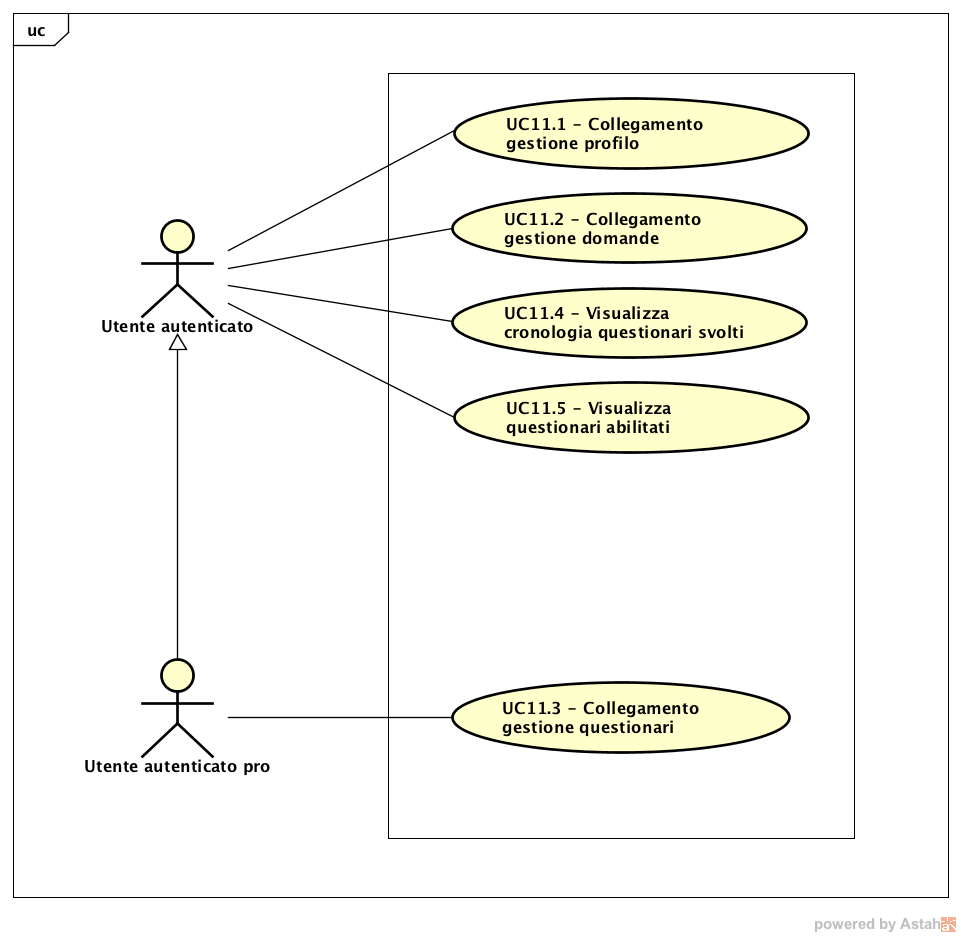
\includegraphics[scale=0.5]{UML/UC11.png}
	\caption{UC11: Gestione pagina utente}
\end{figure}

\begin{itemize}
\item\textbf{Attori}: utente autenticato, utente autenticato pro;
\item\textbf{Descrizione}: da questa pagina l'attore può: 
\begin{itemize}
	\item Visualizzare tutti i dati del proprio profilo;
	\item Visualizzare le statistiche dei questionari svolti;
	\item Visualizzare la cronologia dei questionari svolti;
	\item Accedere alla parte del sistema che permette di modificare il profilo;
	\item Accedere alla parte del sistema che permette di aggiungere nuove domande;
	\item Accedere alla parte del sistema che permette di creare questionari.
\end{itemize}
\item\textbf{Precondizione}: l'attore visualizza la pagina iniziale;
\item\textbf{Postcondizione}: l'attore ha visualizzato i suoi dati come richiesto al sistema;
\item\textbf{Scenario principale}: si verifica uno dei seguenti scenari:
\begin{itemize}
\item L'attore sceglie di andare alla pagina di gestione del profilo (UC11.1);
\item L'attore sceglie di andare alla pagina di gestione delle domande (UC11.2);  
\item L'attore sceglie di andare alla pagina di gestione dei questionari (UC11.3);
\item L'attore sceglie di andare alla pagina di visualizzazione della cronologia dei questionari svolti (UC11.4);
\item L'attore sceglie di andare alla pagina di visualizzazione dei questionari abilitati (UC11.5);
\end{itemize}
\item\textbf{Inclusioni}: Viene incluso l'UC7 per la compilazione dei questionari.
\end{itemize}

\subsubsection{Caso d'uso UC11.1: Collegamento gestione profilo}
\begin{itemize}
\item\textbf{Attori}: utente autenticato, utente autenticato pro;
\item\textbf{Descrizione}: l'attore viene portato nella pagina di gestione del profilo dove potrà modificare liberamente tutti i suoi dati;
\item\textbf{Precondizione}: l'attore ha premuto l'apposito link di gestione del profilo;
\item\textbf{Postcondizione}: il sistema ha portato l'attore alla pagina di gestione del profilo;
\item\textbf{Scenario principale}: l'attore si trova nella pagina di gestione del profilo e potrà attuare tutte le modifiche desiderate.
\end{itemize}

\subsubsection{Caso d'uso UC11.2: Collegamento gestione delle domande}
\begin{itemize}
\item\textbf{Attori}: utente autenticato, utente autenticato pro;
\item\textbf{Descrizione}: l'attore viene portato nella pagina di gestione delle domande dove potrà inserire o modificare le sue domande;
\item\textbf{Precondizione}: l'attore ha premuto l'apposito link di gestione delle domande;
\item\textbf{Postcondizione}: il sistema ha portato l'attore alla pagina di gestione delle domande;
\item\textbf{Scenario principale}: l'attore si trova nella pagina di gestione delle domande e potrà attuare tutte le modifiche desiderate.
\end{itemize}

\subsubsection{Caso d'uso UC11.3: Collegamento gestione questionari}
\begin{itemize}
\item\textbf{Attori}: utente autenticato, utente autenticato pro;
\item\textbf{Descrizione}: l'attore viene portato nella pagina di gestione dei questionari dove potranno compiere tutte le azioni possbili sui questionari;
\item\textbf{Precondizione}: l'attore ha premuto l'apposito link di gestione dei questionari;
\item\textbf{Postcondizione}: il sistema ha portato l'attore alla pagina di gestione dei questionari;
\item\textbf{Scenario principale}: l'attore si trova nella pagina di gestione dei questionari e potrà attuare tutte le modifiche desiderate.
\end{itemize}

\subsubsection{Caso d'uso UC11.4: Visualizzazione cronologia questionari svolti}
\label{UC11.4}
\begin{figure}[h]
	\centering
	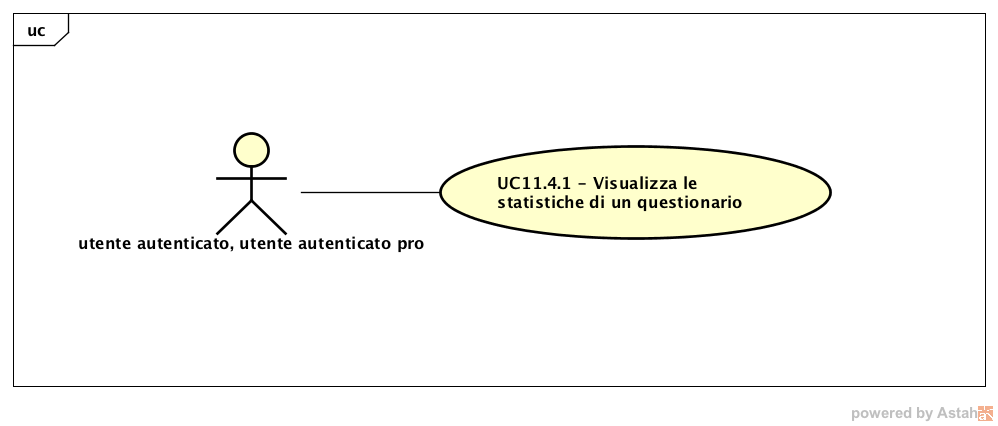
\includegraphics[scale=0.5]{UML/UC11_4.png}
	\caption{UC11.4: Visualizzazione cronologia questionari svolti}
\end{figure}
\begin{itemize}
\item\textbf{Attori}: utente autenticato, utente autenticato pro;
\item\textbf{Descrizione}: l'attore può visualizzare la cronologia dei questionari svolti;
\item\textbf{Precondizione}: l'attore ha compilato almeno un questionario;
\item\textbf{Postcondizione}: il sistema ha mostrato all'attore la cronologia dei questionari;
\item\textbf{Scenario principale}: l'attore ha scelto di visualizzare le statistiche di un questionario (UC11.4.1).
\end{itemize}

\subsubsection{Caso d'uso UC11.4.1: Selezione e visualizzazione delle statistiche di un questionario scelto}
\begin{itemize}
\item\textbf{Attori}: utente autenticato, utente autenticato pro;
\item\textbf{Descrizione}: l'attore può selezionare un questionario fra quelli presenti e quindi visualizzarne le statistiche;
\item\textbf{Precondizione}: il sistema mostra all'attore tutti i questionari da lui svolti;
\item\textbf{Postcondizione}: il sistema ha mostrato all'attore le statistiche del questionario selezionato;
\item\textbf{Scenario principale}: l'attore si trova nella pagina dedicata alla visualizzazione delle statistiche di un particolare questionario da lui scelto.
\end{itemize}

\subsubsection{Caso d'uso UC11.5: Visualizzazione questionari abilitati}
\label{UC11.5}
\begin{figure}[h]
	\centering
	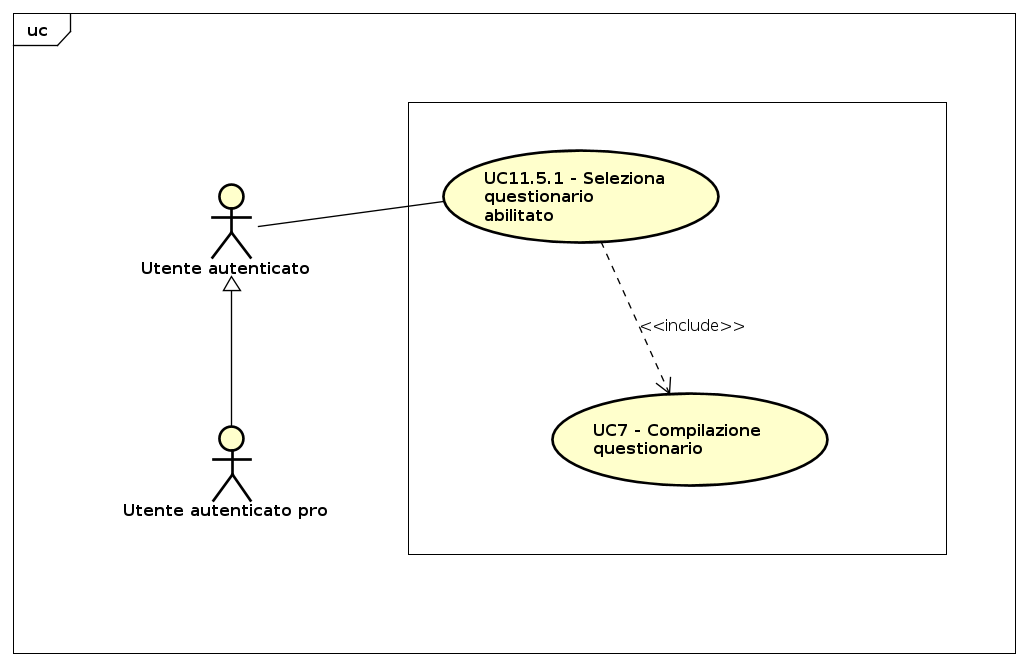
\includegraphics[scale=0.5]{UML/UC11_5.png}
	\caption{UC11.5: Visualizza questionari abilitati}
\end{figure}
\begin{itemize}
\item\textbf{Attori}: utente autenticato, utente autenticato pro;
\item\textbf{Descrizione}: l'attore può visualizzare la lista dei questionari a cui è stato abilitato da parte dell'utente autenticato pro proprietario del questionario.
\item\textbf{Precondizione}: l'attore deve aver richiesto l'abilitazione ad un questionario e deve essere stato accettato dal proprietario;
\item\textbf{Postcondizione}: il sistema ha mostrato all'attore tutti i questionari a cui è stato abilitato;
\item\textbf{Scenario principale}: l'attore ha selezionato un questionario abilitato (UC11.5.1).
\end{itemize}

\subsubsection{Caso d'uso UC11.5.1: Seleziona questionario abilitato}
\begin{itemize}
\item\textbf{Attori}: utente autenticato, utente autenticato pro;
\item\textbf{Descrizione}: l'attore può selezionare un questionario a cui è stato abilitato ed eseguirlo;
\item\textbf{Precondizione}: l'attore deve essere stato abilitato ad almeno un questionario;
\item\textbf{Postcondizione}: l'attore ha selezionato un questionario a cui è stato abilitato e il sistema è pronto per farlo eseguire;
\item\textbf{Scenario principale}: l'attore richiede di eseguire un questionario a cui è stato abilitato.
\end{itemize}